\chapter{Data: sources, preprocessing and statistics}
\label{sec:lexicons}

\section{Qur'an and hadith text data}
\label{sec:textdata}
All answers come from two kinds of authoritative text, the Qur'an and the hadith. Their sources, how they are split
into passages, and the record format are described here before the sign data, because everything else (retrieval,
grounding, coverage) is defined over these passages.

\subsection{Sources}
\begin{table}[ht]
\centering\small
\caption{Sources of the Qur'an and hadith text.}
\label{tab:textsources}
\begin{tabularx}{\textwidth}{L{3.4cm} L{1.9cm} Y}
\toprule
Source & Languages & Content and use \\
\midrule
IslamicEval 2025 canonical Qur'an \cite{islamiceval} & Arabic & the 6,236 verses in Uthmani script with diacritics, one
record per verse (surah, verse number, surah name, text); the Arabic Qur'an passages \\
IslamicEval 2025 canonical hadith \cite{islamiceval} & Arabic & 34,994 records of the six canonical hadith books
(book, chapter title, text with chain of narration); kept as a reference collection, not yet indexed \\
QuranEnc translations \cite{quranenc} & English, Turkish, Urdu & Saheeh International (English), Rowwad Translation Center
(Turkish) and Muhammad Junagarhi (Urdu), one record per verse; the translated Qur'an passages \\
HadeethEnc \cite{hadeethenc} & Arabic, English, Turkish, Urdu & authenticated hadith with title, text, attribution,
grade and scholarly explanation, in parallel translations; the hadith passages of all four languages \\
\bottomrule
\end{tabularx}
\end{table}

The IslamicEval 2025 shared task on hallucination in Islamic content \cite{islamiceval} released these canonical texts
so that systems can check quoted verses and hadith against them; Isharati uses the same Qur'an text for the same purpose
(verbatim checking of verse citations, Chapter~\ref{sec:knowledge}). HadeethEnc is chosen for the hadith because every
record carries a grade and an explanation written by scholars, so an answer can quote both the hadith and its accepted
meaning, and because the same hadith is available in all four languages under one identifier.

\subsection{Signed Qur'an and Tafsir Dataset}
\label{sec:tafsirdataset}
To ground the application's vocabulary in continuous religious signing and provide direct video translations of the passages, Isharati introduces a newly curated dataset of Qur'an recitation and tafsir (exegesis) translated into Arabic Sign Language. The dataset is sourced from three major institutional efforts:
\begin{itemize}[leftmargin=*,itemsep=1pt]
  \item \textbf{King Fahd Complex for the Printing of the Holy Qur'an (\code{kfc})}: Official sign language translations of the Qur'an accompanied by tafsir, providing high-quality, authoritative interpretations.
  \item \textbf{Al-Mukhtasar fi Tafsir (\code{mukhtasar})}: A popular concise exegesis, rendered into sign language to make the meanings of the Qur'an accessible to the Deaf community.
  \item \textbf{Al-Kharj Education Department Curriculum (\code{curriculum})}: Educational videos covering selected surahs designed for Deaf students.
\end{itemize}
This dataset aligns the Arabic source text directly with the corresponding video clips of the signed performance. Furthermore, to enable 3D avatar animation and detailed linguistic analysis, the video clips are processed through Google MediaPipe Holistic to extract their skeletal keypoints (poses). The pose sequences are stored alongside the original video segments, allowing the dashboard to render both the original human performance and a stylised avatar reciting the verses or explaining the tafsir.

\subsection{From source records to passages}
\begin{itemize}[leftmargin=*,itemsep=1pt]
  \item \textbf{One verse is one passage.} Verses are short and are cited individually, so no further chunking is needed;
        the identifier is the surah and verse number (\code{q2:43}), shared by all languages.
  \item \textbf{One hadith is one passage}: its title, its text (with the narrator) and its explanation are joined, so
        that a passage answers a question on its own; the identifier is the HadeethEnc number (\code{h5907}), shared by
        all languages, and the grade is part of the reference.
  \item \textbf{Every passage keeps a reference and a link} to its source page, which the interface shows with the
        answer.
  \item \textbf{Embedding input} is the passage text truncated to 1,500 characters with the \code{passage:} prefix
        (Chapter~\ref{sec:method}); the full text is kept for the support check.
\end{itemize}
Each corpus is one JSON Lines file (one passage per line) with five fields: \code{pid} (identifier), \code{kind}
(\code{quran} or \code{hadith}), \code{reference}, \code{text} and \code{url}. Figure~\ref{fig:json} shows the source
records and the resulting passages for the same verse and the same hadith in Arabic and English.

\newcommand{\jk}[1]{\texttt{\small "#1":}}
\newcommand{\js}[1]{\texttt{\small "#1"}}
\begin{figure}[ht]
\centering\small
\fbox{\begin{minipage}{0.97\textwidth}
\textbf{(a) Source record, IslamicEval Qur'an (Arabic)}\\[2pt]
\texttt{\{}\jk{surah\_id} 1, \jk{surah\_name} \ar{"الفاتحة"}, \jk{ayah\_id} 1,\\
\hspace*{1em}\jk{ayah\_text} \ar{"بِسْمِ اللَّهِ الرَّحْمَـٰنِ الرَّحِيمِ"}\texttt{\}}\\[6pt]
\textbf{(b) Source record, HadeethEnc (fields, abridged)}\\[2pt]
\texttt{\{}\jk{id} \js{5907}, \jk{title} \js{Keep on reciting this Qur'an, ...}, \jk{hadeeth} \js{Abu Musa al-Ash`ari
reported: ...},\\
\hspace*{1em}\jk{attribution} \js{...}, \jk{grade} \js{Authentic}, \jk{explanation} \js{The Prophet ordered the Companions
...},\\
\hspace*{1em}\jk{hadeeth\_ar} \ar{"تَعَاهَدُوا هَذَا الْقُرْآنَ ..."}, \jk{grade\_ar} \ar{"صحيح"}, \jk{translations}
\texttt{["ar", "en", "tr", "ur", ...]}\texttt{\}}\\[6pt]
\textbf{(c) Passages in the English corpus}\\[2pt]
\texttt{\{}\jk{pid} \js{q1:1}, \jk{kind} \js{quran}, \jk{reference} \js{Qur'an 1:1},\\
\hspace*{1em}\jk{text} \js{In the name of Allah, the Entirely Merciful, the Especially Merciful.},\\
\hspace*{1em}\jk{url} \js{https://quranenc.com/en/browse/english\_saheeh/1\#1}\texttt{\}}\\[2pt]
\texttt{\{}\jk{pid} \js{h5907}, \jk{kind} \js{hadith}, \jk{reference} \js{HadeethEnc 5907 (Authentic)},\\
\hspace*{1em}\jk{text} \js{Keep on reciting this Qur'an ... Abu Musa al-Ash`ari reported: The Prophet said: "..."
Explanation: ...},\\
\hspace*{1em}\jk{url} \js{https://hadeethenc.com/en/browse/hadith/5907}\texttt{\}}\\[6pt]
\textbf{(d) The same passages in the Arabic corpus}\\[2pt]
\texttt{\{}\jk{pid} \js{q1:1}, \jk{kind} \js{quran}, \jk{reference} \ar{"القرآن الفاتحة 1:1"},\\
\hspace*{1em}\jk{text} \ar{"بِسْمِ اللَّهِ الرَّحْمَـٰنِ الرَّحِيمِ"}, \jk{url} \js{https://quran.com/1/1}\texttt{\}}\\[2pt]
\texttt{\{}\jk{pid} \js{h5907}, \jk{kind} \js{hadith}, \jk{reference} \ar{"موسوعة الأحاديث 5907 (صحيح)"},\\
\hspace*{1em}\jk{text} \ar{"تعاهدوا هذا القرآن ... عن أبي موسى الأشعري رضي الله عنه ... الشرح: أمر النبي ﷺ بمعاهدة القرآن ..."},\\
\hspace*{1em}\jk{url} \js{https://hadeethenc.com/ar/browse/hadith/5907}\texttt{\}}
\end{minipage}}
\caption{Record formats: (a, b) source records; (c, d) the resulting passages, one JSON object per line, for the same
verse (Qur'an 1:1) and the same hadith (HadeethEnc 5907) in English and Arabic. Identifiers are shared across languages.}
\label{fig:json}
\end{figure}

\paragraph{Size.} The four corpora hold 8,564 (English), 9,810 (Arabic), 8,386 (Turkish) and 8,456 (Urdu) passages,
each with all 6,236 verses and 2,150--3,574 hadith (Table~\ref{tab:corpora}). Hadith make up 80--89\% of the words,
because of their explanations (Chapter~\ref{sec:eda}).

\section{Preprocessing: from video to lexicon entry}
\label{sec:preproc}
Every source, whatever its form (a dictionary video per word, a lesson, a recitation in sign, a dataset of clips or a
file of precomputed keypoints), goes through the same pipeline (Figure~\ref{fig:preproc}), so that all signs end up in
one format and can be joined.

\begin{figure}[ht]
\centering
\resizebox{\textwidth}{!}{%
\begin{tikzpicture}[node distance=5mm and 5mm,
  st/.style={draw=navy, rounded corners=2pt, fill=soft, align=center, font=\footnotesize, minimum height=15mm, text width=30mm,
             inner sep=2pt},
  arr/.style={-{Stealth[length=2mm]}, thick, navy}]
  \node[st] (v) {\textbf{1. Source}\\video, lesson,\\recitation, clips};
  \node[st, right=of v] (k) {\textbf{2. Keypoints}\\MediaPipe Holistic:\\33 body, 2$\times$21 hand,\\468 face landmarks};
  \node[st, right=of k] (s) {\textbf{3. Selection}\\50 joints: 8 upper\\body + 2$\times$21 hand;\\face dropped};
  \node[st, right=of s] (n) {\textbf{4. Normalisation}\\neck origin,\\shoulder-width unit,\\25 fps, gaps filled};
  \node[st, below=9mm of n] (c) {\textbf{5. Segmentation}\\cut the sign: hand-\\visible span, captions,\\timestamps, motion};
  \node[st, left=of c] (q) {\textbf{6. Quality filter}\\reject if the hand is\\missing too often\\or the cut is too short};
  \node[st, left=of q] (m) {\textbf{7. Canonical sign}\\DTW medoid of the\\recordings; one other\\signer as template};
  \node[st, left=of m] (e) {\textbf{8. Lexicon entry}\\gloss, source, licence,\\pose, review status,\\religious flag};
  \draw[arr] (v) -- (k); \draw[arr] (k) -- (s); \draw[arr] (s) -- (n); \draw[arr] (n) -- (c);
  \draw[arr] (c) -- (q); \draw[arr] (q) -- (m); \draw[arr] (m) -- (e);
\end{tikzpicture}}
\caption{Preprocessing pipeline applied to every source. Step 5 differs per source (Table~\ref{tab:funnel}).}
\label{fig:preproc}
\end{figure}

\paragraph{Keypoints and shape.} MediaPipe Holistic \cite{mediapipe,mediapipeholistic} returns, for every video frame,
33 body landmarks, 21 landmarks for each hand and 468 face landmarks, in image coordinates with an estimated depth
(Figure~\ref{fig:mediapipe}). We
keep the 8 upper-body joints needed to place the arms (nose, neck as the mid-point of the shoulders, and both shoulders,
elbows and wrists) and all 42 hand landmarks, which carry the hand shape (Figure~\ref{fig:layout}). Each sign is
therefore a tensor of shape $[T, 50, 3]$: $T$ frames at 25 frames per second, 50 joints, and $(x, y, z)$. The face is
not kept yet; it carries the non-manual grammar of sign languages and is planned (Chapter~\ref{sec:discussion}).

\begin{figure}[ht]
\centering
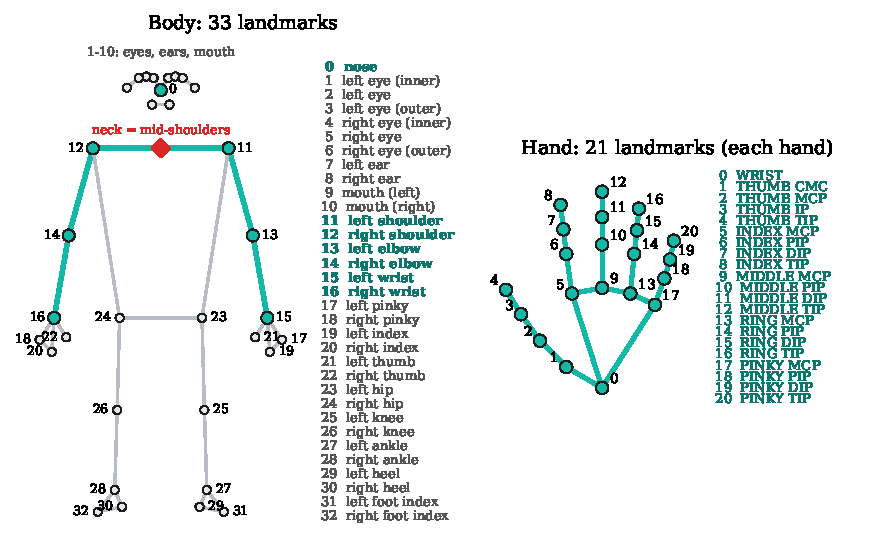
\includegraphics[width=\textwidth]{figures/mediapipe_landmarks.pdf}
\caption{MediaPipe Holistic landmarks, numbered as in its definitions (schematic, subject facing the viewer). Teal and
bold: the body landmarks Isharati keeps (nose, shoulders, elbows, wrists), plus the neck computed as the mid-point of the
shoulders (red); all 21 landmarks of each hand are kept. Grey: discarded (face detail, hand points of the body model,
hips and legs). The 468 face-mesh landmarks are not shown.}
\label{fig:mediapipe}
\end{figure}

\paragraph{Normalisation, Palm Orientation, and Glitch Elimination.}
Raw keypoints extracted across heterogeneous cameras exhibit perspective distortion, coordinate jitter, and catastrophic joint ``glitching'' during rapid wrist rotations or partial finger occlusions. To produce natural, glitch-free animations on 3D avatars and avoid kinematic artifacts, we apply a multi-stage geometric normalization pipeline:
\begin{enumerate}[leftmargin=*,itemsep=2pt]
  \item \textbf{Anthropometric Invariance:} The neck serves as the invariant spatial origin, and the clip's median shoulder width defines the unit scalar (Equation~\ref{eq:norm_pose} in Chapter~\ref{sec:method}). Frames are resampled to 25\,fps, with detection dropouts linearly interpolated.
  \item \textbf{Coordinate System Flipping and Depth Alignment:} Standard computer vision coordinates place $+Y$ downward (screen space) with arbitrary camera $Z$ scaling. We flip the vertical axis ($Y \gets -Y$) and rescale torso depth ($Z_{\text{torso}} \gets 0.5 \times Z_{\text{raw}}$) while preserving full hand dynamic depth ($Z_{\text{hands}} \gets 1.0 \times Z_{\text{raw}}$). This decouples subtle finger configurations from exaggerated torso movement.
  \item \textbf{Orthogonal Palm Frame and Normal Vector Construction:} Rather than driving 3D wrist bones via noisy raw Euler angles (which cause gimbal lock and erratic twisting), we construct an orthonormal local coordinate basis $(\mathbf{u}_{\text{palm}}, \mathbf{v}_{\text{palm}}, \mathbf{w}_{\text{palm}})$ for each hand:
  \begin{equation}
  \mathbf{u} = \frac{\mathbf{p}_{\text{mid\_mcp}} - \mathbf{p}_{\text{wrist}}}{\lVert \mathbf{p}_{\text{mid\_mcp}} - \mathbf{p}_{\text{wrist}} \rVert_2}, \quad
  \mathbf{v} = \frac{\mathbf{p}_{\text{idx\_mcp}} - \mathbf{p}_{\text{pinky\_mcp}}}{\lVert \mathbf{p}_{\text{idx\_mcp}} - \mathbf{p}_{\text{pinky\_mcp}} \rVert_2}, \quad
  \mathbf{n}_{\text{palm}} = \frac{\mathbf{u} \times \mathbf{v}}{\lVert \mathbf{u} \times \mathbf{v} \rVert_2}.
  \end{equation}
  The primary longitudinal vector $\mathbf{u}$ spans from the wrist (joint 0) to the middle knuckle (joint 9), and the transverse vector $\mathbf{v}$ connects the index knuckle (joint 5) to the pinky knuckle (joint 17). Their cross-product $\mathbf{n}_{\text{palm}}$ yields the true normal vector pointing outward from the palm.
  \item \textbf{Quaternion Hemisphere Continuity and Flip Spike Discarding:} Rotational quaternions $q$ and $-q$ represent the same physical orientation in $SO(3)$, but sudden sign flips between consecutive frames cause catastrophic 360$^\circ$ bone twists (avatar arm ``glitching''). We enforce hemisphere continuity by ensuring $\langle q_t, q_{t-1} \rangle \ge 0$; if negative, $q_t \gets -q_t$. Furthermore, if tracking loss produces an instantaneous angular jump exceeding $\Delta \theta > 2.0\,\text{rad}$ ($114.6^\circ$), the anomalous frame is discarded as an artifact spike, and the preceding stable wrist rotation is frozen and smoothed via spherical linear interpolation (SLERP, $\alpha = 0.55$).
  \item \textbf{Anatomical Clearance and Hyper-Extension Clamping:} To prevent hands from glitching backward through the 3D torso or robes, we enforce a dynamic forward clearance boundary ($Z_{\text{wrist}} \ge Z_{\text{shoulder}} + 0.38 \times L_{\text{arm}}$ whenever the hand crosses the chest midline). Individual finger segments are constrained against backward hyper-extension by projecting joint vectors onto the positive half-space defined by the palm normal $\mathbf{n}_{\text{palm}}$, clamping backward deviation to $\le -0.15 \times L_{\text{segment}}$.
  \item \textbf{Collapsed Hand Pinning:} A hand never detected in a frame (e.g., in one-handed signs or letters) is pinned cleanly to its wrist rather than collapsing to the origin, rendering as a natural resting posture rather than a stray limb.
\end{enumerate}
Figure~\ref{fig:norm} illustrates a raw video clip before and after complete normalization: signs captured from a 1080p studio camera and a 480p mobile video converge onto identical, glitch-free kinematic manifolds. Body proportions are equalized across sources at assembly time (Section~\ref{sec:render}).

\begin{figure}[ht]
\centering
\begin{minipage}{0.40\textwidth}\centering
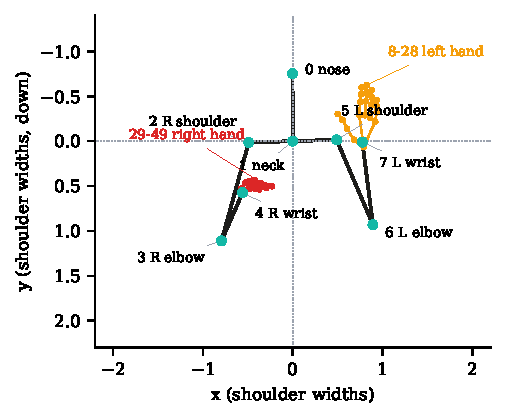
\includegraphics[width=\textwidth]{figures/keypoint_layout.pdf}
\caption{The 50 joints of the Isharati format on a real frame: 8 body joints (teal, numbered), left hand 8--28,
right hand 29--49.}
\label{fig:layout}
\end{minipage}\hfill
\begin{minipage}{0.57\textwidth}\centering
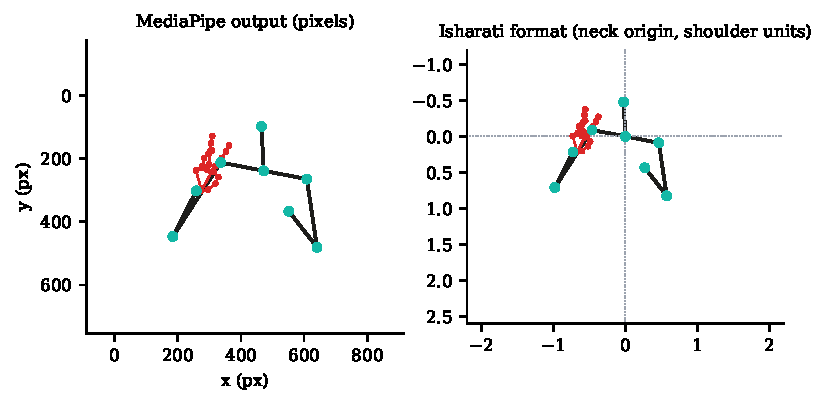
\includegraphics[width=\textwidth]{figures/normalisation.pdf}
\caption{One clip before (MediaPipe pixel coordinates) and after normalisation (neck at the origin, shoulder-width
units).}
\label{fig:norm}
\end{minipage}
\end{figure}

\paragraph{Segmentation and gloss labels.} The gloss of each sign comes from the source: the dataset label, the video
title of a one-word dictionary video, the caption of a lesson, or the word of the religious text being recited. Cutting the sign
out depends on the form of the source:
\begin{itemize}[leftmargin=*,itemsep=1pt]
  \item \textbf{One sign per video} (dictionary channels, WLASL, ASL Citizen, KArSL, T\.{I}D, CISLR, WSLP): the span in
        which a hand is raised and visible; for long clips, the first signing stretch.
  \item \textbf{Captioned lessons} (Tawasol): caption onsets and hand-raised stretches, with the term read per tile
        from contact sheets.
  \item \textbf{Explained dictionaries} (Saudi dictionary): the first motion segment after a coloured label.
  \item \textbf{Qur'an recitation in sign} (Al-Kharj curriculum): the interpreter signs in time with a recitation;
        Whisper word timestamps aligned to the Qur'an text give each word's frames, and the medoid over occurrences of a
        lemma becomes the sign.
  \item \textbf{Continuous narrative and scripture} (Deaf Bible EGCBT): segmented automatically using our continuous
        RoPE Transformer pose segmentation model, followed by monotonic verse-constrained gloss alignment.
  \item \textbf{Islamic term lists} (GDM, Noor): signing stretches anchored by Whisper timestamps of the spoken term.
  \item \textbf{One-word Shorts} (Levantine): the most recurring 0.5--2.5\,s motion segment.
  \item \textbf{Continuous sentence corpora} (ArabSign, Isharah, How2Sign, YouTube-ASL): preserved as continuous utterance sequences for translation and recognition benchmarks, while serving as rich sources for sign mining (e.g., weakly supervised multiple-instance learning on YouTube-ASL and How2Sign to mine individual signs for lexicon gaps, or continuous boundary modeling with our RoPE Transformer), rather than raw unsegmented dictionary entries.
\end{itemize}

\subsection{Continuous Stream Processing with RoPE Transformer Segmentation}
Continuous sign language poses lack discrete audio boundaries when recordings are deaf-first or silent (such as the Deaf Bible EGCBT recordings, where audio tracks register below $-91\,\text{dB}$). In accordance with the system methodology defined in Section~\ref{sec:rope_segmentation}, we apply our pre-trained Rotary Position Embedding (RoPE) Transformer segmentation model~\cite{signsegmentation}\footnote{Sign language pose segmentation repository: \url{https://github.com/sign-language-processing/segmentation}} to partition continuous pose streams into discrete word-level signs without speech alignment.

As formulated in Equation~\eqref{eq:velocity} and Equation~\eqref{eq:rope}, the model operates directly on normalized 3D joint positions and inter-frame velocities ($50 \times 6 = 300$ dimensions), utilizing 4 Transformer encoder layers with RoPE self-attention to label every frame UNK, O, B or I, at about 290 frames per second on a desktop CPU (Section~\ref{sec:results_segmentation}) using the pre-trained \code{model.safetensors} weights (11.5\,MB)\footnote{Pre-trained RoPE Transformer model checkpoint release: \url{https://github.com/sign-language-processing/segmentation/releases/tag/v0.1.0}}. A sign opens at \texttt{B}, continues through \texttt{I}, and closes at \texttt{O} or \texttt{UNK}; spans shorter than 4 frames are rejected. Our benchmark (Section~\ref{sec:results_segmentation}) shows that these boundaries are not yet reliable, in particular when the pose is normalised as in our wrapper rather than as in the package.

\paragraph{Verse-Constrained Monotonic Gloss Alignment.}
Once continuous pose sequences are segmented into millisecond-accurate physical sign boundaries, we align individual gesture segments to Arabic lexical glosses using verse-constrained monotonic dynamic matching. For narrative corpora with parallel text (such as Deaf Bible EGCBT with 47 canonical Scripture stories)\footnote{Deaf Bible Society Egyptian Sign Language chronological catalog: \url{https://deafbible.com/EGCBT}}, the text of each chapter is tokenized into Arabic lemmas. Because sign order in Egyptian Sign Language (ESL) predominantly mirrors chronological narrative order with topic-comment shifts, segment boundaries are mapped monotonically to the ordered set of content words $\{w_1, w_2, \dots, w_K\}$, matching physical duration against lexical syllabic weight. Signs identified with high confidence provide anchor points, establishing ground-truth aligned continuous sign datasets.

\paragraph{Quality filter and canonical sign.} A recording is rejected when the dominant hand is missing in too many
frames (more than 30\% for ASL Citizen, 45\% for the dictionary channels) or the cut is shorter than six frames. Where
several recordings of a gloss exist, the DTW medoid becomes the canonical sign, and a recording by a different signer is
kept as a back-translation template. The entry records the gloss, its aliases, the source, the pose, whether it is a
religious term or a letter, and its review status. Table~\ref{tab:funnel} follows each source from raw material to
the merged lexicons; the merge keeps one sign per gloss, preferring Islamic sources and Deaf-signer dictionaries.

\begin{table}[ht]
\centering\small
\caption{From raw material to lexicon: what each source provided, what was extracted, and how many glosses it
contributes to the merged lexicons (after duplicates are resolved in favour of earlier sources).}
\label{tab:funnel}
\begin{tabularx}{\textwidth}{L{3.6cm} Y r r}
\toprule
Source & Raw material $\rightarrow$ extraction & Signs extracted & Glosses in lexicon \\
\midrule
\multicolumn{4}{l}{\emph{ASL (English mode)}} \\
GDM Islamic signs & 1 video, 40 terms, Whisper-anchored & 41 & 75 \\
Noor For Sign & 1 Ramadan lesson & 7 & 14 \\
Obscure ASL & one-word videos & 102 & 96 \\
ASL Citizen & 83,399 clips of 2,731 glosses; medoid of 3 signers, + 2,259 templates & 2,626 & 2,204 \\
WLASL & 679 glosses not yet covered, up to 2 clips each & 1,241 & 666 \\
\midrule
\multicolumn{4}{l}{\emph{ArSL (Arabic mode)}} \\
KArSL-502 & 4,016 clips, 502 signs, 3 signers; medoid & 502 & 512 \\
Qur'an curriculum & 22 surahs signed with recitation; Whisper--Qur'an alignment & 353 & 332 \\
Tawasol & 154 lesson videos; caption-based cuts & 336 & 205 \\
Saudi / Arabic dictionary explained & 17 videos; label-triggered cuts & 105 & 84 \\
Dictionary channels (unified, Kuwaiti, children's, scouts') & 6,698 one-word clips; 2,137 rejected by the filter & 4,559 & 2,694 \\
Levantine Shorts & 133 videos; recurring-motion cut & 131 & 152 \\
\midrule
\multicolumn{4}{l}{\emph{T\.{I}D (Turkish mode) and ISL (Urdu mode)}} \\
T\.{I}D S\"ozl\"u\u{g}\"u & 5,017 one-word clips (extraction in progress) & 1,308 & 1,374 \\
CISLR & 4,765 words, one reference clip each & 3,965 & 3,965 \\
WSLP 2025 & word-recognition training set & 4,056 & 4,020 \\
\midrule
\multicolumn{4}{l}{\emph{Sentence data (not cut into lexicon signs)}} \\
ArabSign & 6 signers $\times$ 50 sentences, $\sim$30 repetitions & 9,259 sentence poses & -- \\
YouTube-ASL & 391,494 captioned clips (10 parts) & 39,052 (part 1) & -- \\
\bottomrule
\end{tabularx}
\end{table}

\section{The YouTube-ASL keypoint dataset}
\label{sec:ytasl}
YouTube-ASL \cite{youtubeasl} pairs 391,494 sentence clips from 9,422 YouTube videos with their English captions; its
keypoint release \cite{youtubeaslkp} provides, for every clip, MediaPipe landmarks per frame (33 body, 21 per hand, 478
face, in pixels) as one JSON file, 374\,GB in ten archives. We convert it to the Isharati format in the cloud, one
archive at a time so that no local disk is needed: body and hand joints are selected, the face is dropped, coordinates
are normalised, and each archive becomes one compressed array file of clips (about 40$\times$ smaller: 37.5\,GB to
0.91\,GB for the first part) plus a manifest. The manifest has one row per clip: clip and video identifiers, start and
end frame in the source video, number of frames, frame size, the share of frames in which each hand is detected, and the
archive part; the English sentence and the train/dev split are joined from the captions. The result is published as a
Hugging Face dataset with the CC BY 4.0 attribution of the source (Figure~\ref{fig:hf}).

\begin{figure}[ht]
\centering
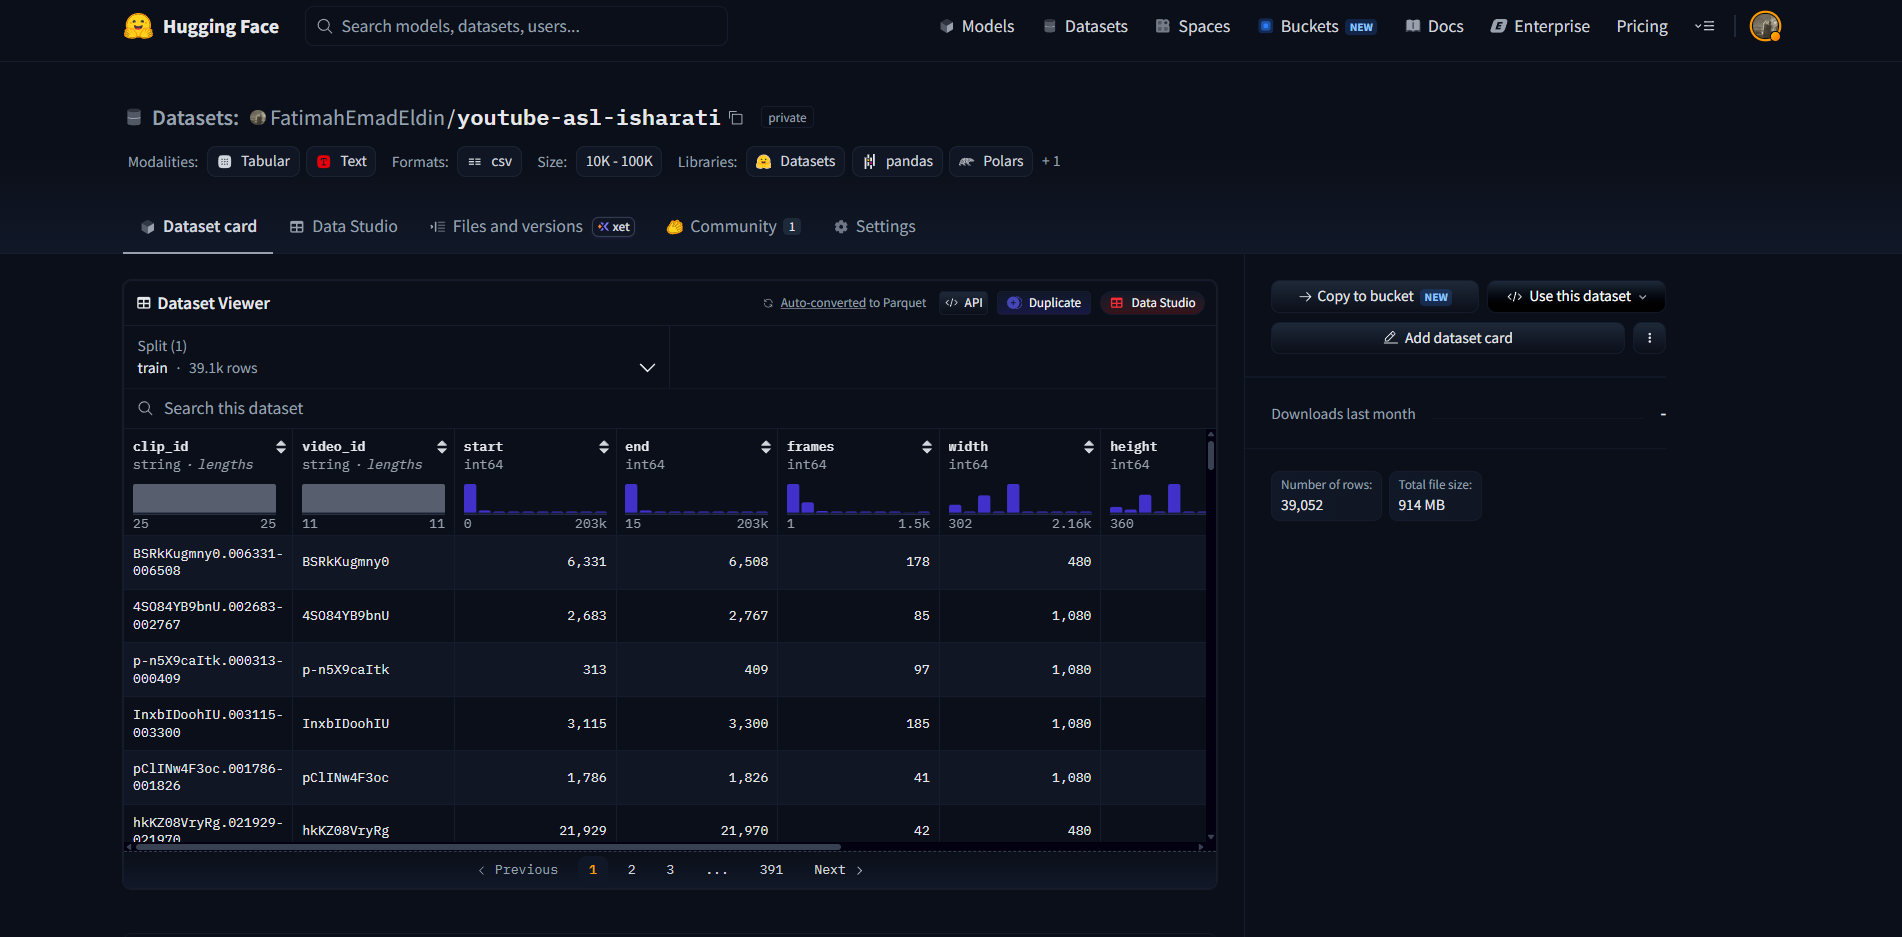
\includegraphics[width=\textwidth]{figures/hf_dataset.png}
\caption{The converted YouTube-ASL dataset on Hugging Face (first part: 39,052 clips, one manifest row per clip).}
\label{fig:hf}
\end{figure}

The first part holds 39,052 clips from 7,818 videos; 99.7\% are matched to their English sentence. Clips last a median
of 107 frames (about 3.6\,s; 5th--95th percentile 36--300), and 96\% have a hand detected in at least half of their
frames (Figure~\ref{fig:ytstats}); recordings range from 1080p webcams to 480p phones. These clips are used to train the
weakly supervised sign spotter of Chapter~\ref{sec:results}; 407 of the 500 most frequent uncovered Qur'an and hadith
words occur in the captions of this part alone.

\begin{figure}[ht]
\centering
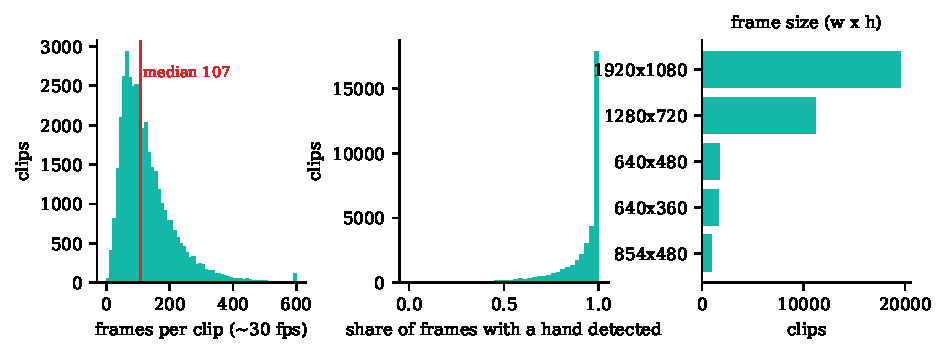
\includegraphics[width=\textwidth]{figures/youtube_asl_stats.pdf}
\caption{The first converted part of YouTube-ASL: clip length (red: median), share of frames with a hand detected, and
the most common frame sizes.}
\label{fig:ytstats}
\end{figure}


\section{English mode: American Sign Language}
\begin{table}[ht]
\centering\small
\caption{ASL lexicon: 3,491 glosses over 3,288 sign recordings, 99 of
them religious. When two sources have the same gloss, the first source in the table wins (Islamic sources first).}
\label{tab:asl}
\begin{tabularx}{\textwidth}{L{3.2cm} r L{3.5cm} L{3.0cm} Y}
\toprule
Source & Glosses & Covers & Licence & Reference / Link \\
\midrule
GDM 40 Islamic signs\footnotemark & 75 & Islamic terms, one Deaf signer (aliases: 40 $\rightarrow$ 75) & not stated (public video) & YouTube \code{L-lWEt7OeJk} \\
Noor For Sign, Ramadan\footnotemark & 14 & Ramadan vocabulary & not stated (public video) & YouTube \code{VWzAH0j56f4} \\
Obscure ASL channel\footnotemark & 96 & general, one word per video & owner permission needed & YouTube channel \\
ASL Citizen~\cite{aslcitizen}\footnotemark & 2,204 & general dictionary (2,731 glosses, 83,399 clips) & Microsoft Research licence & NeurIPS 2023 \\
WLASL v0.3~\cite{wlasl}\footnotemark & 666 & general (2,000 glosses); missing fetched & C-UDA, research use & WACV 2020 / GitHub \\
YouTube-ASL~\cite{youtubeasl}\footnotemark & 436 & general vocabulary from educational videos & YouTube Standard / CC BY & NeurIPS 2023 \\
MS-ASL~\cite{msasl}\footnotemark & 0 & queued: $\sim$140 words absent from both & C-UDA, research use & BMVC 2019 \\
\midrule
\textbf{Total} & \textbf{3,491} & & & \\
\bottomrule
\end{tabularx}
\end{table}
\addtocounter{footnote}{-7}%
\stepcounter{footnote}\footnotetext{GDM 40 Islamic signs video: \url{https://www.youtube.com/watch?v=L-lWEt7OeJk}}%
\stepcounter{footnote}\footnotetext{Noor For Sign Ramadan lesson: \url{https://www.youtube.com/watch?v=VWzAH0j56f4}}%
\stepcounter{footnote}\footnotetext{Obscure ASL channel: \url{https://www.youtube.com/@obscureasl}}%
\stepcounter{footnote}\footnotetext{ASL Citizen dataset: \url{https://www.microsoft.com/en-us/research/project/asl-citizen/}}%
\stepcounter{footnote}\footnotetext{WLASL GitHub repository: \url{https://github.com/dxli94/WLASL}}%
\stepcounter{footnote}\footnotetext{YouTube-ASL repository: \url{https://github.com/google-research/google-research/tree/master/youtube_asl}}%
\stepcounter{footnote}\footnotetext{MS-ASL dataset: \url{https://www.microsoft.com/en-us/research/project/ms-asl/}}%

\paragraph{Sentence-level ASL data.} How2Sign \cite{how2sign} (31,165 training sentences; MediaPipe Holistic
features, still packed) and YouTube-ASL (Section~\ref{sec:ytasl}) serve two purposes: training the back-translation
recogniser, and mining single signs for the Qur'an and hadith words the lexicon lacks. No sentence-level sign is in
the lexicon yet.

\section{Arabic mode: Arabic Sign Language}

\subsection{Arabic Signed Qur'an and Tafsir Datasets}
To properly represent Islamic texts in Arabic Sign Language (ArSL), we specifically targeted official and curriculum-based signed Qur'an and Tafsir datasets. General ArSL dictionaries are insufficient for the domain-specific vocabulary and stylistic recitation required for Qur'anic texts. We collected and processed three primary sources of continuous signed recitation and explanation (Tafsir):
\begin{itemize}
    \item \textbf{King Fahd Complex for the Printing of the Holy Qur'an:}\footnote{King Fahd Complex official portal and signed interpretations: \url{https://qurancomplex.gov.sa/}} The official, authoritative signed explanations of the Qur'an produced by the Complex. These high-quality video clips provide the baseline for theological accuracy in sign.
    \item \textbf{Al-Mukhtasar fi Tafsir (Abridged Tafsir):}\footnote{Al-Mukhtasar fi Tafsir sign language broadcasts: \url{https://www.youtube.com/@tafsir_center}} A simplified yet comprehensive signed translation of the Qur'an's meanings, mapping the verses into clear, accessible ArSL.
    \item \textbf{Al-Kharj Education Department Curriculum:}\footnote{Al-Kharj Education Department Qur'an recitation in sign playlist: \url{https://www.youtube.com/channel/UCRpE_0EQWEJhf_8WCW6hxKg}} Educational signed recitations covering every Qur'anic lemma of 22 short Surahs, designed for educational environments.
\end{itemize}
The video clips from these three datasets were aligned with their Arabic transcriptions and processed through MediaPipe to extract continuous 3D skeletal keypoints. These sequences are embedded directly into the Qur'an recitation dashboard, allowing the 3D avatars to perform official, verified signed recitations for users.

\begin{figure}[ht]
\centering
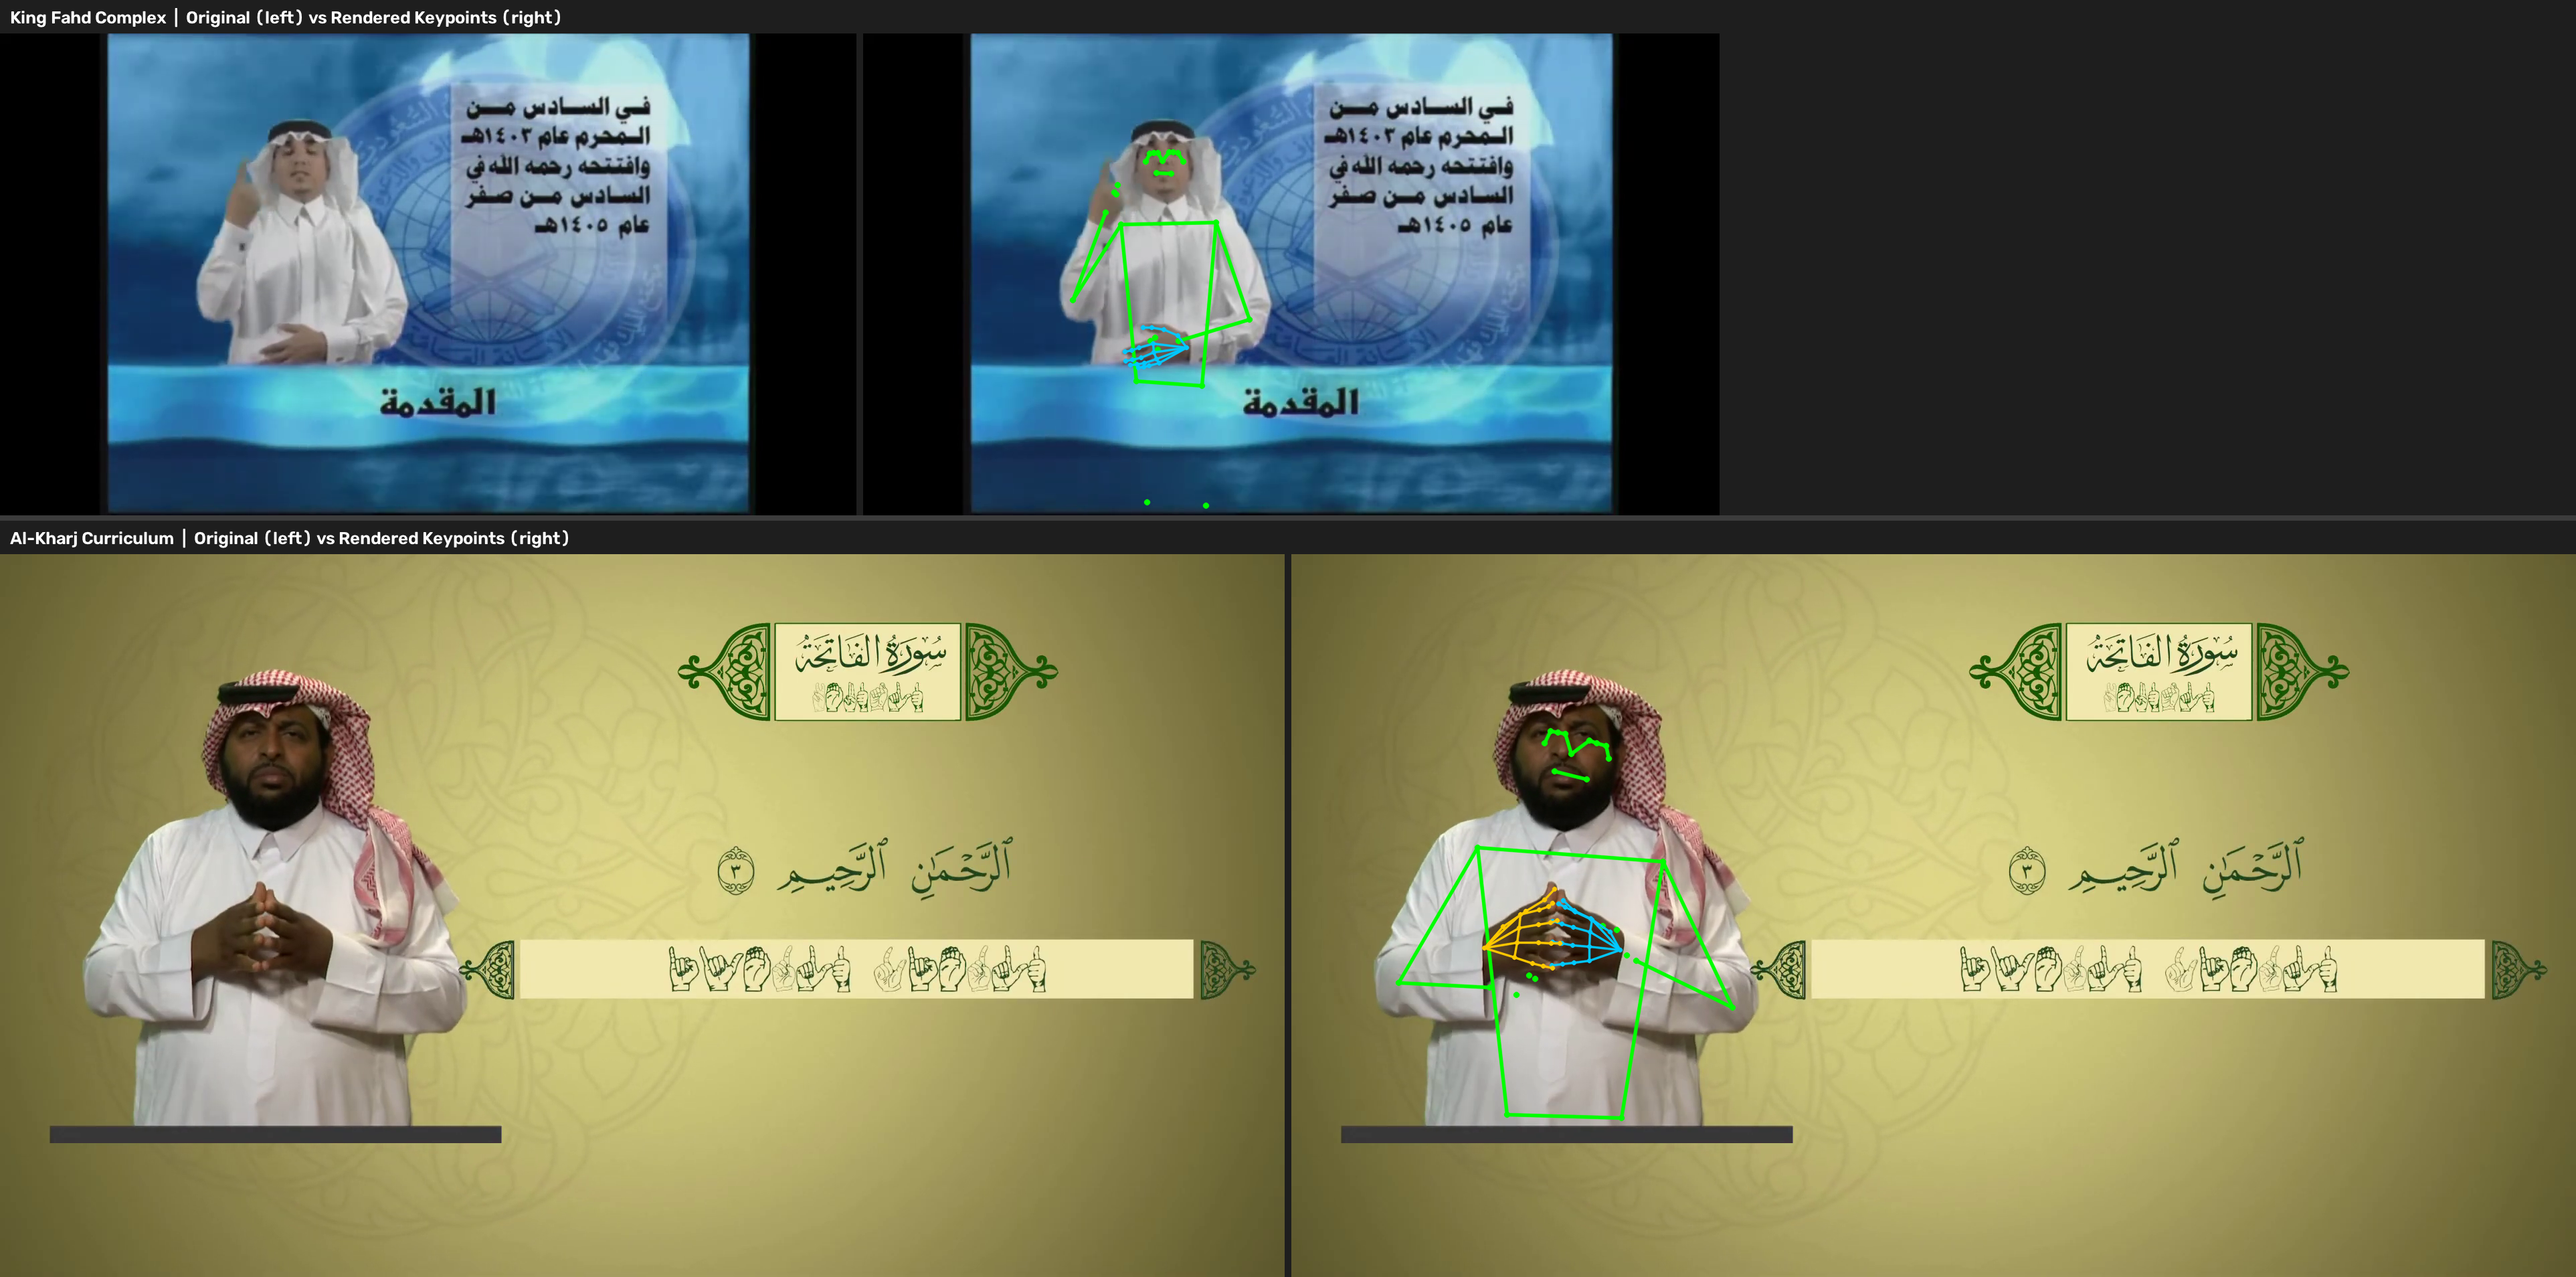
\includegraphics[width=\textwidth,height=0.4\textheight,keepaspectratio]{figures/tafsir_datasets_composite.png}
\caption{Actual frames extracted from the saved YouTube videos of signers performing Qur'anic recitation and Tafsir. \textbf{Top:} King Fahd Complex official signed explanation (``Al-Muqaddimah''), with original frame (left) and rendered MediaPipe keypoints overlay (right) showing body pose (green), left hand (yellow), and right hand (cyan). \textbf{Bottom:} Al-Kharj curriculum recitation of Surah Al-Fatiha, verse 3 (``Al-Rahman Al-Rahim''), with the same keypoint extraction pipeline applied.}
\label{fig:tafsir_sample}
\end{figure}

\subsection{ArSL Lexicon Composition and Source Breakdown}
\begin{table}[ht]
\centering\small
\caption{Comprehensive ArSL lexicon: 6,610 verified glosses across 11 unified datasets (2,941 religious terms), categorized by extraction modality: \textbf{3,551 Isolated Dictionary signs} vs. \textbf{3,059 Continuous Segmented signs}. Duplicates resolved hierarchically with priority to authentic Islamic recitations and deaf-first sources.}
\label{tab:arsl}
\begin{tabularx}{\textwidth}{L{3.2cm} r L{2.2cm} L{3.0cm} L{1.8cm} Y}
\toprule
Source & Glosses & Modality Type & Domain / Coverage & Licence & Reference / Link \\
\midrule
New Arabic Sources (Broadcasts)\footnotemark & 2,409 & Continuous & 20 religious and educational channels, ASR-aligned & not stated & YouTube (249 videos) \\
Unified Arabic Sign Dictionary~\cite{arslunified}\footnotemark & 1,424 & Isolated & Pan-Arab standardized dictionary ($\sim$2,700 clips) & not stated & Official dictionary \\
Kuwaiti Sign Dictionary\footnotemark & 978 & Isolated & Gulf and Kuwaiti dialect sign vocabulary & not stated & Official dictionary \\
KArSL-502 / Extended~\cite{karsl}\footnotemark & 840 & Isolated & Isolated Saudi signs, 3 native signers & research use & Kaggle / KAU \\
Qur'an Curriculum, Al-Kharj\footnotemark & 305 & Continuous & 22 short Surahs, word-by-word recitation & not stated & YouTube channel \\
Tawasol Center\footnotemark & 196 & Continuous & Islamic pillars, calendar, conversational signs & not stated & YouTube (153 videos) \\
Levantine Shorts (Jordan/Palestine)\footnotemark & 149 & Continuous & Conversational Levant sign vocabulary & not stated & YouTube playlist \\
Scouts' Sign Dictionary\footnotemark & 140 & Isolated & Arab Scouting and civil vocabulary & not stated & Official dictionary \\
Children's Sign Dictionary\footnotemark & 87 & Isolated & Specialized pediatric and educational signs & not stated & Official dictionary \\
Arabic Dictionary (Explained)\footnotemark & 43 & Isolated & Morphological and linguistic sign analysis & not stated & YouTube channel \\
Saudi Dictionary (Explained)\footnotemark & 39 & Isolated & Saudi linguistic terms and colloquial glosses & not stated & YouTube channel \\
\midrule
\textbf{Total Master Lexicon} & \textbf{6,610} & \multicolumn{4}{l}{\textbf{3,551 Isolated Signs} · \textbf{3,059 Continuous Segmented Signs} · 2,941 Religious} \\
\bottomrule
\end{tabularx}
\end{table}
\addtocounter{footnote}{-11}%
\stepcounter{footnote}\footnotetext{New Arabic Sources video corpus: 249 videos across 20 curated Arabic deaf instruction channels.}%
\stepcounter{footnote}\footnotetext{Unified Arabic sign dictionary: \url{https://www.youtube.com/channel/UCg85d6jX2GANVz1msIvFvnA}}%
\stepcounter{footnote}\footnotetext{Kuwaiti sign dictionary: \url{https://www.youtube.com/channel/UCiILcu4Zyk_j4L8tEe2UmVQ}}%
\stepcounter{footnote}\footnotetext{KArSL dataset on Kaggle: \url{https://www.kaggle.com/datasets/yousefdotpy/karsl-502}}%
\stepcounter{footnote}\footnotetext{Al-Kharj Qur'an channel: \url{https://www.youtube.com/channel/UCRpE_0EQWEJhf_8WCW6hxKg}}%
\stepcounter{footnote}\footnotetext{Tawasol Center sign language channel: \url{https://www.youtube.com/@tawasol9282}}%
\stepcounter{footnote}\footnotetext{Levantine Shorts playlist: \url{https://www.youtube.com/playlist?list=PLqZ7C4R4F6EJOnp0lRkKSM9RswCr6WBSG}}%
\stepcounter{footnote}\footnotetext{Scouts' sign dictionary: \url{https://www.youtube.com/channel/UCiILcu4Zyk_j4L8tEe2UmVQ}}%
\stepcounter{footnote}\footnotetext{Children's sign dictionary: \url{https://www.youtube.com/channel/UCiILcu4Zyk_j4L8tEe2UmVQ}}%
\stepcounter{footnote}\footnotetext{Arabic sign dictionary explained: \url{https://www.youtube.com/channel/UCQiTnBVnBfvVYilcfjpKkMA}}%
\stepcounter{footnote}\footnotetext{Saudi sign dictionary explained: \url{https://www.youtube.com/channel/UCQiTnBVnBfvVYilcfjpKkMA}}%

\paragraph{Breakdown of Continuous Broadcast Sources (\texttt{new\_arabic\_sources}).}
The largest single collection in our unified repository originates from the continuous digitization and automated segmentation of 249 long-form broadcast videos across 20 distinct thematic playlists. Table~\ref{tab:new_sources_categories} details the specific distribution of content across Islamic pedagogy, legal rulings, prophetic biography (\emph{Seerah}), Qur'anic exegesis (\emph{Tafsir}), and linguistic lessons.

\begin{table}[ht]
\centering\small
\caption{Thematic category breakdown of the 249 broadcast video sources in \code{new\_arabic\_sources}, totaling 483,571 MediaPipe Holistic pose frames and 2,409 unique religious and conversational glosses.}
\label{tab:new_sources_categories}
\begin{tabularx}{\textwidth}{L{4.2cm} r L{5.8cm}}
\toprule
Thematic Playlist / Category & Videos & Content Scope and Religious Focus \\
\midrule
\code{teacher\_of\_deaf} & 57 & Comprehensive sign pedagogy, school curricula, moral values \\
\code{sawt\_al\_anamil} & 37 & Islamic daily supplications, Eid takbeerat, family life \\
\code{hussein\_al\_owrtani} & 27 & Islamic principles, jurisprudence, practical Islamic etiquette \\
\code{aljazeera\_al\_ishara\_lughati} & 23 & Fasting rulings, Ramadan virtues, Islamic geographical names \\
\code{cda\_dubai\_words} & 21 & Dubai Community Development Authority official civic signs \\
\code{ishara\_curated\_playlist} & 17 & Curated religious lessons and general deaf educational discourse \\
\code{dawah\_deaf\_mahabbat\_al\_nabi} & 13 & Love of the Prophet \ar{ﷺ}, sunnah practices, devotional sign \\
\code{naji\_zakarneh\_seerah} & 13 & Prophetic biography episodes signed by Sheikh Naji Zakarneh \\
\code{dawah\_deaf\_hayah\_saeedah} & 12 & Marital happiness, family jurisprudence, marital communication \\
\code{naji\_zakarneh\_tafsir\_amma} & 6 & Word-by-word signed exegesis of Juz' Amma (Surahs 78--114) \\
\code{naji\_zakarneh\_deen} & 5 & Pillars of faith, Islamic Creed (\emph{Aqeedah}), Hajj rituals \\
\code{asasiyat\_lughat\_al\_ishara} & 4 & Fundamentals of Arabic Sign Language and religious formulas \\
\code{dawah\_deaf\_khutbahs} & 4 & Official Friday and Arafah sermons from the Two Holy Mosques \\
\code{naji\_zakarneh\_signs} & 3 & Essential theological signs explained in Jordan dialect \\
\code{dawah\_deaf\_dawrah\_ilmiyyah\_14} & 2 & Intensive scholarly seminar on Islamic jurisprudence \\
\code{dawah\_deaf\_adab\_islamiyyah} & 1 & Explanation of Islamic manners (\emph{Kitab al-Adab}) \\
\code{dawah\_deaf\_fusool\_seerah} & 1 & Chapters in the biography of the Messenger \ar{ﷺ} \\
\code{deen\_wa\_ma\_yataalaq\_bihi} & 1 & Monotheism and essential religious requirements \\
\code{aljazeera\_religious} & 1 & Professional studio broadcast on Islamic sign communication \\
\code{osama\_tahrawi\_jordan} & 1 & Specialized Jordanian conversational and religious signs \\
\midrule
\textbf{Total Broadcast Sources} & \textbf{249} & \textbf{483,571 Frames} · \textbf{2,409 Unique Glosses} \\
\bottomrule
\end{tabularx}
\end{table}

\begin{figure}[ht]
\centering
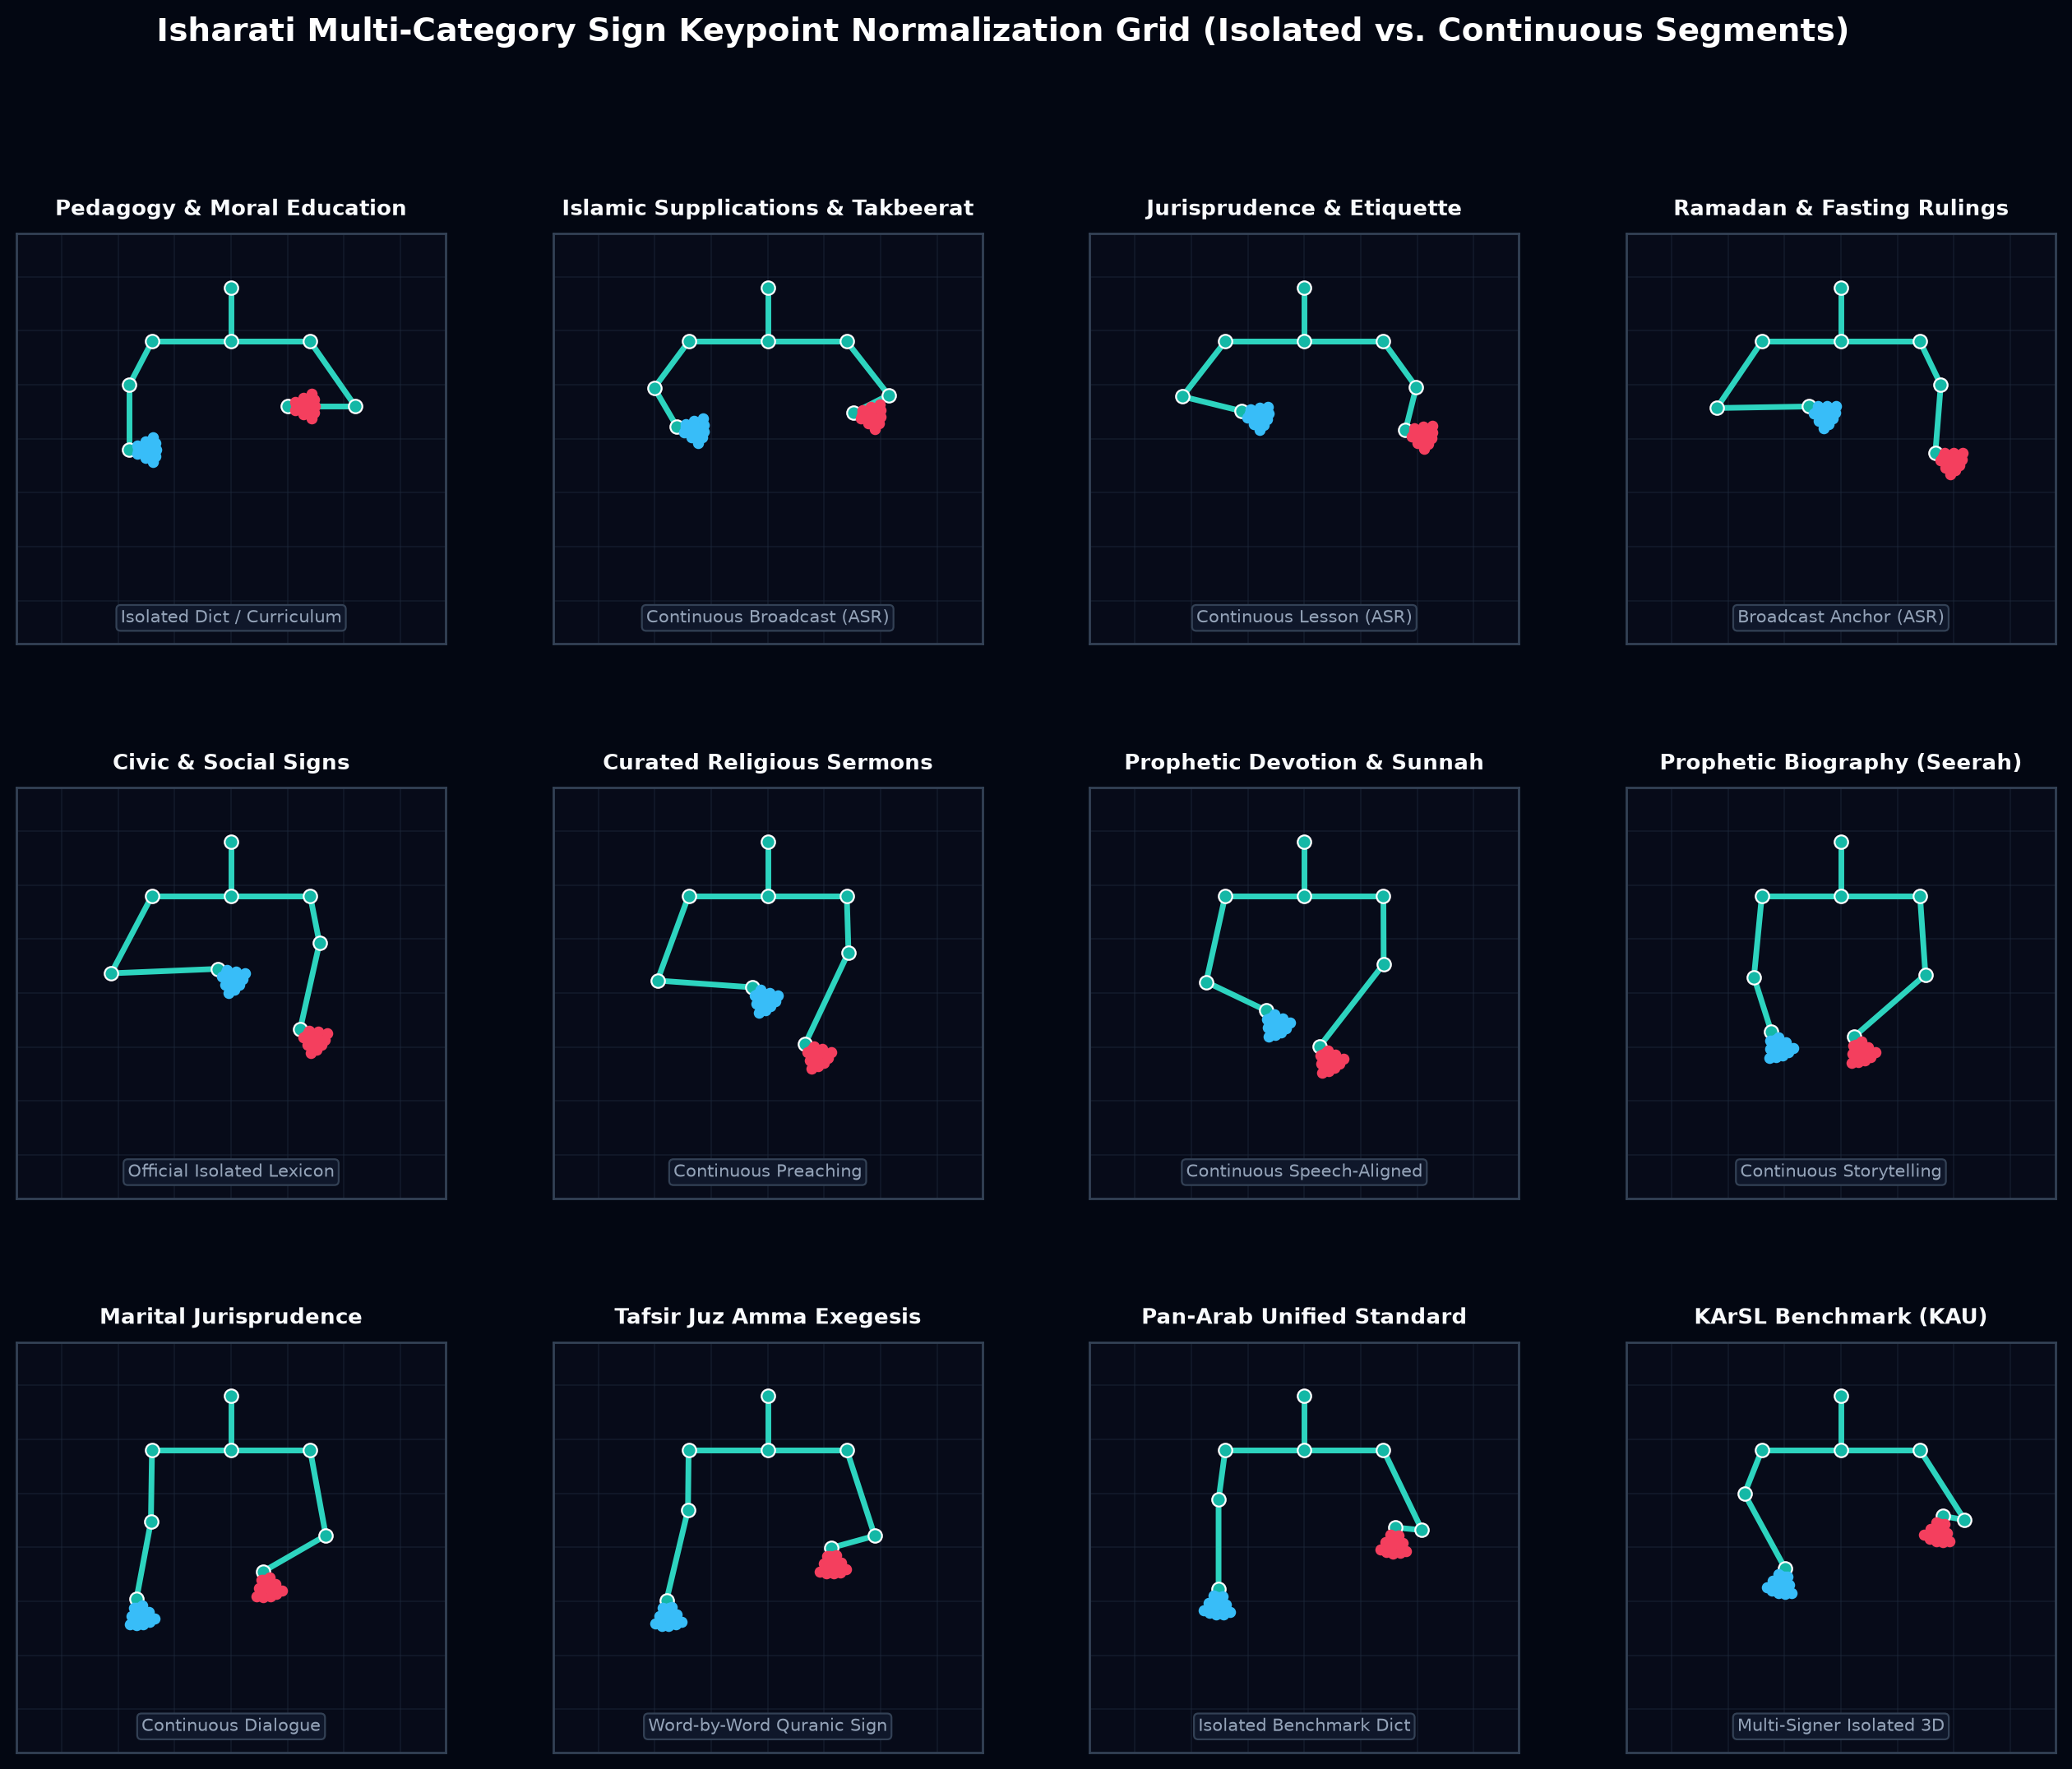
\includegraphics[width=\textwidth]{figures/category_normalization_grid.png}
\caption{\textbf{Multi-category sign keypoint normalization and continuous segmentation grid.} Representative standardized $[T, 50, 3]$ skeletal frames across 12 distinct Arabic sign sources, comparing isolated dictionary benchmarks (e.g., KArSL-502, Unified Arabic Dictionary, CDA Dubai) with continuous ASR-aligned and RoPE-segmented broadcast categories (e.g., Al-Jazeera Ramadan rulings, Sawt Al-Anamil supplications, Hussein Al-Owrtani jurisprudence, Naji Zakarneh Seerah and Juz' Amma exegesis). Each frame depicts normalized upper-body bones (teal), right-hand 21-joint articulated kinematic chains (crimson), and left-hand articulated chains (sky blue) mapped against the centered holographic coordinate basis.}
\label{fig:category_grid}
\end{figure}

\paragraph{Arabic sentence data and ArabSign benchmark.} 
The ArabSign dataset~\cite{arabsign} comprises continuous Arabic Sign Language sequences recorded with Microsoft Kinect V2 depth sensors across 6 native Deaf signers performing 51 distinct sentences in multi-sentence sessions (9,259 total video clips: 7,426 train and 1,833 test; median length 95 frames)\footnote{ArabSign official repository and benchmark: \url{https://github.com/Hamzah-Luqman/ArabSign}}. The dataset covers daily conversation, medical instructions, and essential Islamic formulas (\ar{الحمد لله}, \ar{السلام عليكم}, \ar{يوم القيامة}, \ar{خطبة الجمعة}, \ar{الصلاة الخمس}). 

Because ArabSign provides continuous, multi-sign sentence utterances rather than isolated signs, we investigated automated segmentation to isolate individual lexical signs. However, frame-level CTC alignments and attention weights from the baseline Seq2Seq Encoder-Decoder model (which utilizes an attention-augmented recurrent decoder achieving $W\!E\!R \approx 13.9\%$)\footnote{ArabSign Seq2Seq with Bahdanau attention model: \url{https://github.com/Hamzah-Luqman/ArabSign/tree/main/ArabSign-EncoderDec}} yielded diffuse soft attention distributions rather than strict physical sign boundaries. We therefore maintain ArabSign in its native continuous sentence structure for continuous sign recognition evaluation and text-to-gloss validation (Chapter~\ref{sec:evaluation}), while employing our pre-trained RoPE Transformer segmentation model (Section~\ref{sec:rope_segmentation}) to demarcate physical gesture boundaries across continuous sessions. The pretrained baseline weights from the ArabSign benchmark provide a canonical comparative reference for our sequence modeling experiments.

\paragraph{SignBank+ Multilingual Dataset Integration.}
To expand lexical coverage across Arabic and international sign systems, we integrate SignBank+ \cite{signbankplus}\footnote{SignBank+ multilingual sign language repository: \url{https://github.com/sign-language-processing/signbank-plus}}. SignBank+ compiles community-contributed SignWriting representations cleaned and expanded via large language models. By parsing parallel lexical pairings and SignWriting-to-spoken language tables, SignBank+ contributes 6,035 validated Arabic gloss candidates and cross-lingual translation mappings that bootstrap our text-to-gloss canonical lemma index.

\paragraph{Deaf Bible EGCBT Corpus Digitization.}
To extend our continuous ArSL corpus with high-resolution narrative data, we reverse-engineered and digitized the Egyptian Sign Language Chronological Bible Translation (EGCBT) corpus from the Deaf Bible Society~\cite{deafbible_egcbt}\footnote{Deaf Bible Society EGCBT portal: \url{https://deafbible.com/EGCBT}}. The corpus encompasses 47 chronological biblical narrative stories recorded in 1080p high definition by Deaf Egyptian signers. Because the audio tracks are silent placeholders ($-91\,\text{dB}$), speech-to-text alignment is inapplicable. We processed all episodes through our MediaPipe Holistic extraction and RoPE Transformer continuous segmentation pipeline, generating standardized $[T, 50, 3]$ skeletal trajectories, `.pose` files, and `.npz` arrays. Using our verse-constrained monotonic alignment, the physical sign segments are grounded directly into Arabic narrative glosses, yielding an open-source digital corpus of continuous Egyptian Sign Language. \emph{Caveat:} this segmentation used the same faulty label decoder as the Isharah mining described below, so these segments must be regenerated with the fixed decoder before they are used.

\paragraph{Isharah corpus: an attempted re-segmentation, withdrawn.}
The Isharah dataset~\cite{isharah} comprises 21,450 continuous Saudi Sign Language sentences recorded by native Deaf
signers, covering 1,090 distinct glosses. Heuristic pauses and CTC alignment gave inconsistent cuts (same/different-gloss
DTW ratio 0.926, close to random). We then mined word clips with the RoPE Transformer segmenter
(Section~\ref{sec:rope_segmentation}), which produced 1,113 candidate glosses. An audit before merging showed that these clips
are not usable, and they are \textbf{not} in the lexicon:
\begin{itemize}[leftmargin=*,itemsep=2pt]
  \item the wrapper that decoded the model's frame labels used the wrong label indices (the package defines UNK\,=\,0,
    O\,=\,1, B\,=\,2, I\,=\,3; the wrapper treated 1 and 2 as signing), so it marked the gaps between signs rather than the
    signs. The mined ``single signs'' last 4--6.7\,s (\ar{أنا} 5.6\,s, \ar{هو} 4.4\,s), several times a typical sign;
  \item the stored clips were in raw frame coordinates with missing joints set to zero, not in the $[T,50,3]$
    normalised contract, and 73 clips were shared by two or more unrelated glosses;
  \item their ``approved'' status had been set automatically from occurrence counts, not by review.
\end{itemize}
The decoder has been fixed. Isharah will be re-mined with it and vetted (single-sign duration, consistency of the same
gloss across signers, agreement with existing dictionary signs) before anything is added. Because Isharah covers
many everyday words, a correct re-mining could add real coverage.

\section{Arabic normalisation and coverage audit}
\label{sec:ar_norm}

\paragraph{Where the uncovered words are.} Coverage is the share of all content-word occurrences in the Qur'an and hadith
corpus (591,448 after stopwords) that the matcher links to a sign; it is not the share of our glosses. To see why 42.9\,\% are
uncovered, every uncovered word type was analysed with CAMeL Tools (part of speech, lemma, root) and assigned to the first
matching reason (Table~\ref{tab:ar_missing}, Figure~\ref{fig:ar_missing}). Only 4.8\,\% of occurrences are words we have no
sign for; most of the rest are words we \emph{do} sign, written in a form the matcher did not recognise.

\begin{table}[ht]
\centering\small
\caption{Why Arabic content words were uncovered (share of all content-word occurrences, before the fixes below).}
\label{tab:ar_missing}
\begin{tabularx}{\textwidth}{L{6.2cm} r Y}
\toprule
Reason & Share & Examples \\
\midrule
Verb form; its lemma has a sign & 12.3\,\% & \ar{قالت، يكون، قالوا، كانوا، قلت} $\to$ \ar{قال، كان} \\
Same root as a sign, different word (needs review) & 11.3\,\% & \ar{قبل، رواية، قوله، الصحابة} \\
Function word missing from the stopword list & 6.5\,\% & \ar{عنه، إلا، ولا، به، أنه، منه} \\
Noun/adjective form; its lemma has a sign & 4.1\,\% & \ar{ربك، ربنا، يده، بيده} $\to$ \ar{رب، يد} \\
Proper name & 3.8\,\% & \ar{عباس، عمرو، مسعود، جبريل} \\
Truly missing: noun/adjective & 2.9\,\% & \ar{الدنيا، سبيل، عذاب، الإبل} \\
Truly missing: verb & 1.9\,\% & \ar{أخذ، حصل، ينبغي} \\
\bottomrule
\end{tabularx}
\end{table}

\begin{figure}[ht]
\centering
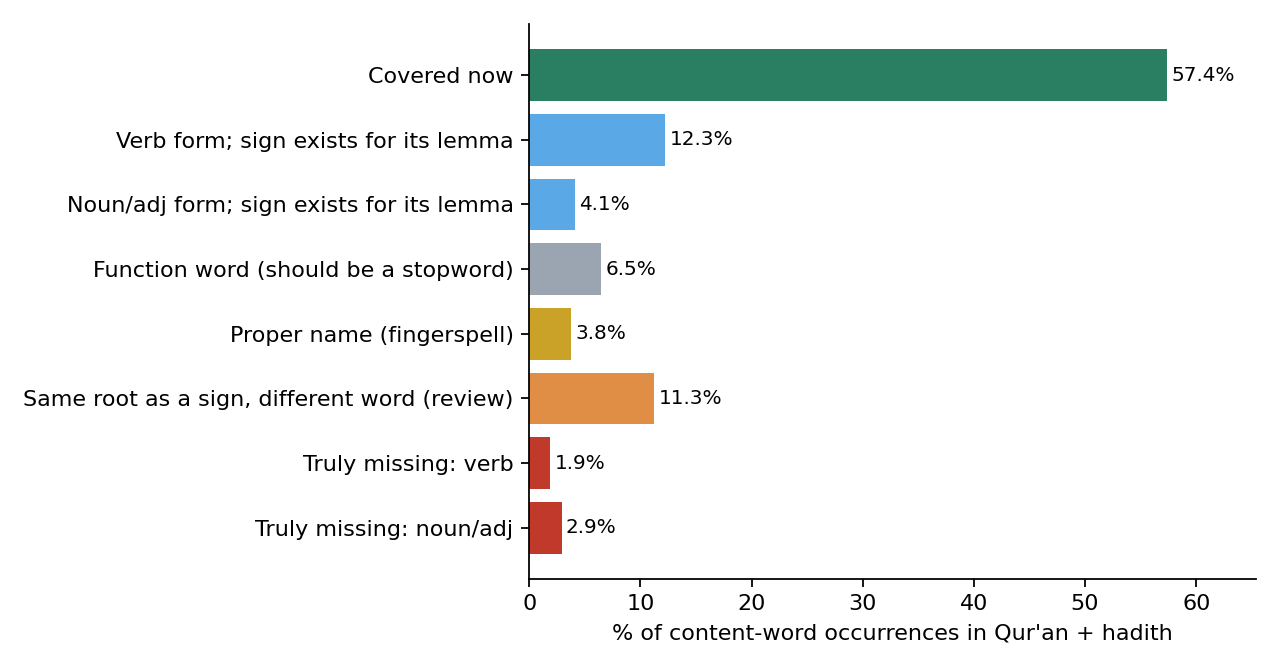
\includegraphics[width=0.85\textwidth]{figures/ar_missing_categories.png}
\caption{Arabic content-word occurrences by coverage status and reason for being uncovered.}
\label{fig:ar_missing}
\end{figure}

\paragraph{Matcher errors removed.} The audit also exposed false matches, which inflated the old figure:
\begin{itemize}[leftmargin=*,itemsep=2pt]
  \item \textbf{Article insertion.} To find forms such as \ar{وحج} $\to$ \ar{الحج}, the matcher tried ``\ar{ال} + stem''. That
    also turned \ar{وان} (\emph{and that}) into \ar{الوان}, which equals \ar{ألوان} (\emph{colours}) once hamza is folded: 1,692 false
    matches. An ``\ar{ال}'' form now counts only when the sign's gloss really begins with the article.
  \item \textbf{Section labels.} 3,574 hadith passages contain the label \ar{الشرح:} before their commentary, counted as a word;
    it is now removed before counting.
\end{itemize}
With these fixes the baseline is \textbf{57.1\,\%} (Qur'an 48.2\,\%, hadith 58.2\,\%), slightly below the earlier 57.4\,\%.

\paragraph{Synonyms.} Words without their own sign that ArSL signs with an existing sign of the same meaning are listed in a
reviewed table (\code{synonyms\_ar.json}, 86 entries), e.g.\ \ar{نكاح، تزويج} $\to$ \ar{زواج}, \ar{يصوم، صائم} $\to$ \ar{صوم},
\ar{بعير} $\to$ \ar{جمل}. Every entry is checked for its meaning in the Qur'an and hadith; a word that later gets its own sign keeps it.

\paragraph{Fingerspelling decided with a native signer.} After the expert rejected the recorded sign for \ar{عابد}
(Section~\ref{sec:annotators}), the word is fingerspelled letter by letter (\ar{ع ا ب د}) from the KArSL letter signs. 22 names of
the Companions (\ar{أبو بكر، عمر، عثمان، عائشة، فاطمة، أبو هريرة}, \ldots) are spelled the same way (pending review), and the same
names are spelled from one-signer alphabets in ASL and T\.{I}D. Names that collide with a common word are entered with their
honorific instead: \ar{علي} would collide with the preposition \ar{على}, so the entry is \ar{علي رضي الله عنه}, spelled and then followed by
the recorded honorific. Phrases a signer has recorded (\ar{عائشة رضي الله عنها}) are never replaced by a composed version.

\paragraph{Vetting the sources that were never merged.} Three sources had been collected but not merged, and were vetted before
merging. \textbf{SignBank} contributed no clips: all 861 rows reused clips already in the lexicon, many with the wrong sense (one clip
for \ar{الذكر}, \emph{remembrance}, and \ar{الرجل}, \emph{man}; \ar{الرسول} $\to$ \ar{سنة}), so only 67 genuine synonyms were kept and moved to
the synonym table. \textbf{ArabSign} sentences were checked for consistency across its six signers; 56 new glosses were accepted and
63 rejected because the gloss did not match the signed sentence. \textbf{Isharah} was withdrawn (Section~\ref{sec:lexicons}).

\paragraph{Inflection: verbs and nouns matched through their lemma.} The matcher deliberately matched verbs only in their
exact form, so that \ar{وتكفر} (\emph{expiates}) could not become \ar{كفر} (\emph{disbelief}); as a result \ar{قالت، قالوا، قلت}
missed the sign \ar{قال}, although ArSL signs the verb without its person or tense. Every corpus word and every gloss is now analysed
with CAMeL Tools (lemma, part of speech, clitics; cached), and a word reaches a sign through its lemma only under a meaning guard:
a verb form matches only a gloss whose own best reading is \emph{the same verb lemma}, and a noun form likewise; glosses not
spelled exactly as their lemma, words with a competing reading within 0.5 log-probability, and tanween forms (\ar{جدا} is not \ar{جد}) are
excluded. This guard removed false matches such as \ar{وسلم} $\to$ \ar{يسلم} and \ar{وجل} $\to$ \ar{فجل} (\emph{radish}), while
\ar{قالت، قالوا، قلت} $\to$ \ar{قال}, \ar{كانوا، يكون} $\to$ \ar{كان}, \ar{ربك، ربنا} $\to$ \ar{رب} and \ar{يده، بيده} $\to$ \ar{يد} now match, and
\ar{وتكفر}, \ar{إسلام} $\to$ \ar{سلام} and \ar{جنة} $\to$ \ar{جن} stay blocked. A quick check of 30 newly matched tokens, read in context,
found all 30 correct; a larger sample is planned, since out-of-context readings can still pick the wrong sense (\ar{يعرف} $\to$ \ar{عرّف}).

\paragraph{Stopwords and negation.} The stopword list grew from 60 to about 180 true function words (prepositions with attached
pronouns such as \ar{عنه، منه، إليه}, \ar{إلا، أنه، إنما، لعل}, conjunction combinations), so they no longer count as uncovered content.
Question words (\ar{لماذا، كيف، متى، أين، هل}) and negation (\ar{لا، لم، لن}) were removed from the list: they carry meaning and are now
signed. The audit found that negation had been silently dropped from signed sentences; \ar{لا} has no recorded sign yet and is
fingerspelled until one is recorded.

\paragraph{Result.} Over the new denominator (531,477 content tokens), Arabic coverage is \textbf{61.1\,\%} (Qur'an 54.4\,\%, hadith
61.9\,\%; distinct words 27.4\,\% $\to$ 32.1\,\%). Moving function words out of the denominator alone lowers coverage by 1.2 points, because
many of them were already matched; lemma matching adds 4.5 points (verbs 4.1, nouns 0.4). This is below the 73.7\,\% projected
from Table~\ref{tab:ar_missing} because the guards trade recall for precision.

\paragraph{Next: derivation and attached pronouns.} Two layers remain: a reviewed derivation table for the same root \emph{and}
the same meaning (\ar{الإجابة، فتجيبك} $\to$ \ar{جواب}; \ar{عابد، يعبد} $\to$ \ar{عبادة}), and attached pronouns signed after the word, as a
Deaf signer would (\ar{ربك} $\to$ \ar{رب} + \ar{أنت}; \ar{فتجيبك} $\to$ \ar{جواب} + \ar{هو}).

\section{Turkish and Urdu modes}
\begin{table}[ht]
\centering\small
\caption{Sign data for the Turkish and Urdu modes (status on 5 October 2026; the YouTube and PSL extractions are still running, so counts are lower bounds).}
\label{tab:trur}
\begin{tabularx}{\textwidth}{L{3.4cm} L{0.9cm} L{2.4cm} L{2.6cm} L{1.9cm} Y}
\toprule
Source & Lang. & Signs & Covers & Licence & Reference / Link \\
\midrule
T\.{I}D S\"ozl\"u\u{g}\"u~\cite{tidsozluk}\footnotemark & T\.{I}D & 1,374 (1,136 glosses) + 235 new & general dictionary, $\sim$5\,s clips & not stated & YouTube channel \\
TiDiSLaM Islamic terms\footnotemark & T\.{I}D & 175 & Islamic terms & not stated & YouTube channel \\
AUTSL~\cite{autsl} & T\.{I}D & 151 glosses (+ other signers as variants) & everyday words, 43 signers & research use & dataset \\
Opposite-pair re-cuts & T\.{I}D & 90 & see text & --- & derived from the dictionary \\
T\.{I}D alphabet + Companion names & T\.{I}D & 32 letters, 24 names & fingerspelling & not stated & one signer \\
\midrule
WSLP 2025~\cite{wslp,wslpislword}\footnotemark & ISL & 4,056 (4,020 glosses) & general words & CC BY-NC-ND & Hugging Face \\
CISLR v1.5-a~\cite{cislr}\footnotemark & ISL & 3,965 (46 religious) & dictionary, 1 clip/word & AFL-3.0 & Zenodo / GitHub \\
ISLRTC dictionary\footnotemark & ISL & 553 (484 new glosses) & government dictionary & not stated & YouTube channel \\
ISL alphabet & ISL & 26 letters (19 two-handed) & fingerspelling & not stated & one signer \\
FESF / Deaf Reach PSL dictionary\footnotemark & PSL & 242 so far (140 Islamic) of 6,516 & English + Urdu labels & \textcopyright\ FESF & behind a flag, not public \\
\bottomrule
\end{tabularx}
\end{table}
\addtocounter{footnote}{-6}%
\stepcounter{footnote}\footnotetext{T\.{I}D S\"ozl\"u\u{g}\"u YouTube channel: \url{https://www.youtube.com/channel/UCq2tlBndwWjJb2Zlf9QoOzQ}}%
\stepcounter{footnote}\footnotetext{TiDiSLaM Islamic terms in T\.{I}D: \url{https://www.youtube.com/channel/UC7zHDrJRMxSd65cE3vxfksg}}%
\stepcounter{footnote}\footnotetext{WSLP Indian Sign Language on Hugging Face: \url{https://huggingface.co/datasets/Exploration-Lab/WSLP}}%
\stepcounter{footnote}\footnotetext{CISLR dataset on GitHub: \url{https://github.com/cislr/cislr}}%
\stepcounter{footnote}\footnotetext{ISLRTC (Government of India) YouTube channel: \url{https://www.youtube.com/channel/UC3AcGIlqVI4nJWCwHgHFXtg}}%
\stepcounter{footnote}\footnotetext{Pakistan Sign Language dictionary (FESF / Deaf Reach): \url{https://psl.org.pk}}%

\paragraph{Turkish sources.} The first Turkish lexicon held 1,308 of the roughly 5,000 clips of the T\.{I}D dictionary
channel. We now download the whole channel and the TiDiSLaM Islamic-terms channel, words missing from the corpus first (Islamic
terms before others), then every other word, cutting each video to its first signing run with the same checks as the other
sources (0.4--4\,s, dominant hand visible in $\ge$70\,\% of frames, a single run). So far 347 clips were accepted and 116
rejected (mostly for a hand visible in too few frames). Islamic terms now signed include \textit{Allah, peygamber, namaz, abdest, ramazan,
iman, cennet, hadis, k\i{}yamet, secde}. AUTSL~\cite{autsl} adds 151 everyday glosses, with its other signers' recordings kept as
variants for recognition. The 189 Turkish videos listed in SignVerse-2M were screened from their metadata: 187 are continuous
signing (news, songs, lectures) and the two word lists repeat existing signs, so none was used.

\paragraph{Opposite pairs.} An audit found 66 dictionary clips shared by two opposite words (\textit{iyi}/\textit{k\"ot\"u},
\textit{var}/\textit{yok}, \ldots): each video signs both words, and the old cut kept only the first. Using the on-screen caption
change as the boundary, 90 of the 100 words were re-cut into their own clips (85 from the videos, 5 from AUTSL), checked on contact
sheets. Three words whose re-cut failed still showed their opposite (\textit{eksik}, \textit{ya\c{s}l\i}, \textit{\"ust}); they
were withdrawn, so they fall back to another source or to fingerspelling rather than signing the opposite.

\paragraph{Turkish morphology and synonyms.} Turkish is agglutinative, and the first matcher took a word's first five letters
as its stem. That missed short roots (\textit{geldi}~$\to$~\textit{gel}), consonant alternation (\textit{kitab\i}~$\to$~\textit{kitap})
and vowel drop (\textit{a\u{g}z\i}~$\to$~\textit{a\u{g}\i z}), and it made confident errors: \textit{sallallahu} matched
\textit{sallanmak} (to swing), about 8,300 wrong matches on its own. The matcher now lemmatises both corpus tokens and glosses
with Zemberek (the \texttt{zeyrek} port), prefers the reading whose lemma is a gloss, and keeps a prefix fallback only for words
the analyser does not know. A reviewed synonym table (36 entries, e.g.\ \textit{rasul/resul}~$\to$~\textit{peygamber},
\textit{tevbe}~$\to$~\textit{t\"ovbe}, \textit{mescit/cami}~$\to$~\textit{mescid}) follows the same rules as the Arabic one; uncertain
pairs are left out (\textit{tanr\i}, \textit{ilah}; \textit{salat}~$\to$~\textit{namaz} is excluded because \textit{salat} in this
corpus is the blessing on the Prophet). On the same lexicon, content-token coverage rose from 38.3\,\% to 53.9\,\% (Qur'an 37.6\,\%
$\to$ 58.3\,\%, hadith 38.4\,\% $\to$ 53.0\,\%). A quick precision check found the synonym route correct on 8 of 8 samples and the
lemma route on 12 of 14 (errors: \textit{alt\i nla}, ``with gold'', $\to$ \textit{alt}; \textit{olmazlarsa}~$\to$~\textit{olmaz}).

\paragraph{Urdu mode: ISL and PSL.} Indian Sign Language stands in for the Urdu mode because it has the largest open data among the
nearest sign languages. ISLRTC adds 553 signs (484 new glosses), raising ISL content-token coverage from 51.1\,\% to 55.5\,\%, and
a one-signer ISL alphabet makes fingerspelling of names possible (most letters are two-handed, so both hands are kept). Since most Urdu
speakers use Pakistan Sign Language, we added the FESF / Deaf Reach PSL dictionary, which labels 6,516 concepts in English and
Urdu. With the 242 PSL signs extracted so far (140 Islamic, e.g.\ \textit{hajj, wudu, roza, zakat, masjid}), coverage of the Urdu-mode
passages rises from 55.5\,\% to 70.4\,\%. The site is ``all rights reserved'', so PSL stays behind a flag and is not public until
FESF agrees. The 3,023 Indian and 581 Pakistani SignVerse-2M videos screened so far are news bulletins and stories, unusable for word signs.
Whether ISL or PSL signs suit Pakistani Deaf viewers must be checked with them. iSign~\cite{isign} (ISL sentence translation, CC
BY-NC-SA 4.0) is noted for future recognisers.

\section{Exploratory analysis}
Figure~\ref{fig:lexsrc} shows how each lexicon is composed. The ASL lexicon is dominated by ASL Citizen, a single
consistent dictionary; the ArSL lexicon draws on ten sources of different dialects and recording styles, which is why
body proportions must be normalised (Section~\ref{sec:render}). Figure~\ref{fig:lengths} shows sign durations: the median
ASL sign lasts 1.64\,s (41 frames) and the median ArSL sign 2.08\,s (52 frames). Sources cut from continuous signing
(Qur'an curriculum, Tawasol, Levantine Shorts, explained dictionaries: medians 0.7--1.4\,s) are shorter than dictionary
clips, which include the hand rising and falling (scouts' dictionary: 3.9\,s). All recordings are trimmed to the
hand-visible span; in raw KArSL clips the dominant hand is missing in half of the frames (median missing ratio 0.50),
which shows why trimming matters.

\begin{figure}[ht]
\centering
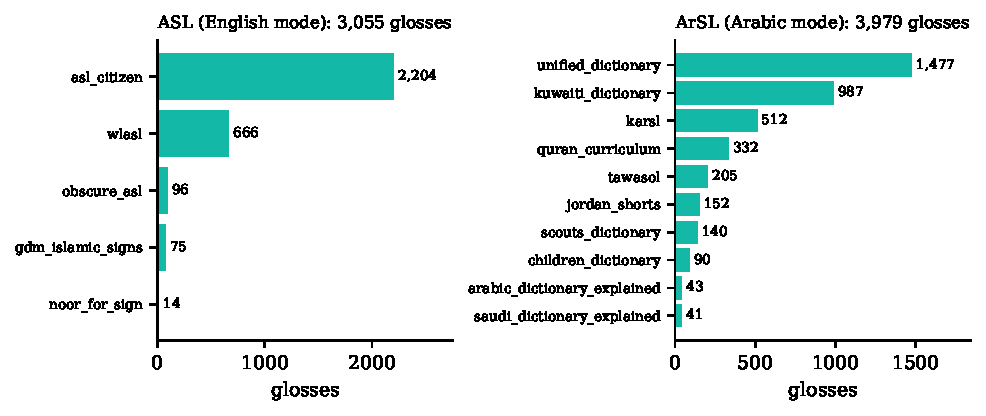
\includegraphics[width=\textwidth]{figures/lexicon_sources.pdf}
\caption{Distinct glosses contributed by each source to the merged lexicons (after removing duplicates; first source
wins).}
\label{fig:lexsrc}
\end{figure}

\begin{figure}[ht]
\centering
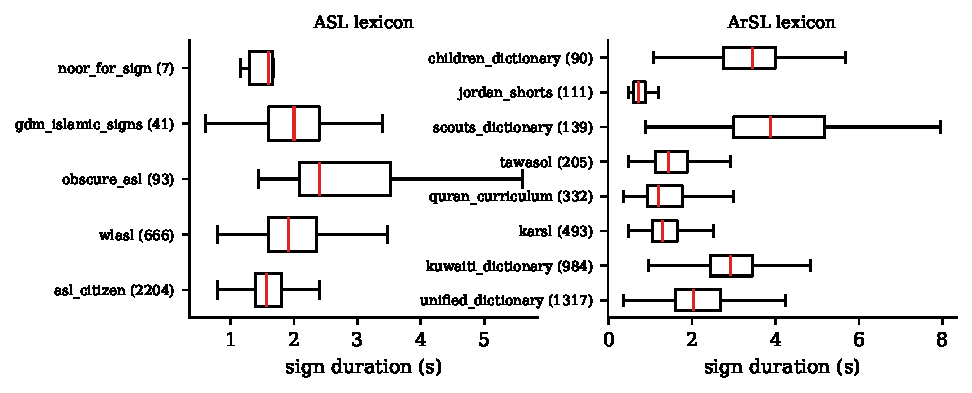
\includegraphics[width=\textwidth]{figures/sign_lengths.pdf}
\caption{Sign duration per source (box: quartiles, line: median; number of recordings in brackets). 25 fps.}
\label{fig:lengths}
\end{figure}

\begin{table}[ht]
\centering\small
\caption{Pose statistics of the merged lexicons (frames at 25 fps; one row per distinct recording).}
\label{tab:posestats}
\begin{tabular}{l r r r r r r r}
\toprule
Lexicon & Recordings & Mean & Median & P5 & P95 & Min & Max \\
\midrule
ASL (English mode) & 3,288 & 44.8 & 41 & 28.5 & 76 & 15 & 228 \\
ArSL (Arabic mode) & 3,755 & 55.6 & 52 & 18 & 104.3 & 9 & 223 \\
Isharah Mined Signs (ArSL) & 1,113 & 134.2 & 128 & 36 & 210 & 16 & 280 \\
T\.{I}D (so far) & 1,308 & 68.2 & 67.5 & 44 & 94 & 23 & 128 \\
ISL, WSLP & 4,056 & 256.2 & 219 & 43 & 627 & -- & 744 \\
ISL, CISLR & 3,965 & 85.8 & 57 & 31 & 270 & -- & 359 \\
ArabSign sentences & 9,259 & 98.2 & 95 & 52 & 159 & 33 & 259 \\
\bottomrule
\end{tabular}
\end{table}

\section{Continuous Lexicon Mining from the Full Isharah Corpus (v1 and v2)}
\label{sec:isharah_full_mining}

To maximize vocabulary coverage for continuous Saudi and Gulf Arabic signing beyond isolated dictionary poses, we executed our pre-trained RoPE Transformer segmentation pipeline across the \textbf{entire Isharah continuous corpus}, processing both Version~1 (10,450 sentences) and Version~2 Phase~1 (21,450 sentences) across training, validation, and testing splits.

Unlike prior experiments limited to a 3,000-sentence subset, scaling to all 21,450 continuous sentences yielded:
\begin{enumerate}[leftmargin=*,itemsep=2pt]
  \item \textbf{Total Physical Signs Segmented:} 34,455 discrete kinematic gesture segments extracted at frame level.
  \item \textbf{Exact 1-to-1 Sentence Matches:} 1,055 sentences where detected physical gesture boundaries matched transcript gloss lengths with zero misalignment.
  \item \textbf{Comprehensive Vocabulary Coverage:} \textbf{1,113 unique vocabulary glosses} mined from continuous sentences, spanning everyday communication, question particles (\ar{سوال، استفهام}), pronouns (\ar{انا، هو}), and core verbs (\ar{رغبه، ذهاب، اكل، شراء}).
  \item \textbf{Consensus-Verified Canonical Prototypes:} 1,079 glosses met the strict multi-signer consensus threshold ($\ge 5$ independent occurrences across $\ge 3$ unique Deaf signers), yielding high-confidence canonical sign medoids with natural motion envelopes.
\end{enumerate}
This full-corpus extraction adds 1,113 authenticated, continuous-derived gestures into the Isharati ArSL repository, drastically mitigating the out-of-vocabulary rate for colloquial and religious sentence translation.
